\chapter{Grundlagen}

\section{Google Design Sprint}
Der Google Design Sprint \ac{GDS} wurde konzipiert, um Organisationen bei der Bewältigung von Herausforderungen und Problemen zu unterstützen. 
Insbesondere die, die durch die dynamische Natur des Marktes und sich verändernde Produktanforderungen entstehen. 
Im Rahmen dieses Konzepts ist es das Ziel, innerhalb eines Zeitraums von fünf Tagen einen Prototyp zu erstellen und zu evaluieren. 
Diese Methode bietet den Vorteil, dass nicht auf die Markteinführung gewartet werden muss, um Feedback zu erhalten. Stattdessen können dringende Fragen sofort beantwortet werden \cite[S.98 f.]{Design_Sprint}.\\
Die fünftägige Methode:\\
Am ersten Tag wird die Grundlage und der Schwerpunkt für die Woche festgelegt. 
Am zweiten Tag konzentriert sich das Team auf die Bewältigung bereits bekannter Herausforderungen. Anders als bei herkömmlichen Brainstorming-Sitzungen arbeiten die Teammitglieder einzeln an Lösungsansätzen und folgen einem strukturierten vierstufigen Prozess, um das kritische Denken zu fördern.
Am dritten Tag muss das Team aus den verschiedenen Lösungsansätzen wählen, welche als Prototyp entwickelt und getestet werden sollen. Dabei kommt die fünfstufige "Sticky Decision"-Methode zum Einsatz, um die besten Lösungen zu identifizieren. Anschließend wird ein detaillierter Prozessplan für den Prototypen erstellt. 
Der vierte Tag ist der Erstellung eines realistischen Prototyps gewidmet, der dann dem Kunden präsentiert werden kann. 
Am letzten Tag wird fünf Kunden in Einzelgesprächen der Prototyp vorgestellt, um ihr Feedback zu erhalten \cite[S.99]{Design_Sprint}.

\section{User Experience}


\section{Technologien}
\subsection{Angular}
Angular ist eine Plattform zur Entwicklung von Webanwendungen, die auf TypeScript \ac{TS} basiert. 
Mit Angular können Single Page Applications für Web-, Mobil- und Desktop-Anwendungen entwickelt werden. 
Es ist Open Source und wird von Google unterstützt, was bedeutet, dass es kostenlos verwendet werden kann und von einer großen Entwickler-Community gepflegt wird. 
Ursprünglich war es als AngularJS bekannt und nutzte JavaScript als Hauptprogrammiersprache. Die Codebasis wurde jedoch komplett neu geschrieben, wobei JavaScript durch TS ersetzt wurde \cite{angular_arch}.\\

\begin{figure}[h]
	\centering
	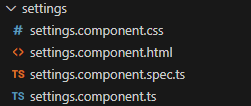
\includegraphics[width=0.5\textwidth]{images/Komponente.png}
	\caption[Komponenten in Angular]{Komponenten in Angular}
	\label{fig:KomponentenAngular}
\end{figure}
Die grundlegenden Bausteine des Angular-Frameworks sind die Komponenten, welche eine isolierte und somit wieder verwendbar Einheit sind. 
Eine Komponente besteht aus einer HTML- und CSS-Datei (siehe Abbildung \ref{fig:KomponentenAngular}), die das Aussehen der Benutzeroberfläche definieren. Die zugehörige Klasse enthält den TS Code, der das Verhalten der Komponente steuert \cite{angular_arch}.\\

\begin{figure}[h]
	\centering
	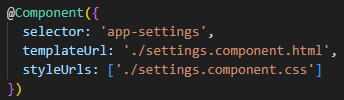
\includegraphics[width=0.5\textwidth]{images/@Component.png}
	\caption[@Component-Dekorator in TS]{@Component-Dekorator in TS}
	\label{fig:@Component}
\end{figure}
Der @Component-Dekorator in TS fügt der Klasse zusätzliche Metadaten hinzu, wie den Pfad zum Template und zu den Styles (siehe templateUrl und styleUrls in der Abbildung \ref{fig:@Component}). Die .spec.ts Datei wird für die Unit-Tests verwendet.
Der Routing-Service ermöglicht die Navigation innerhalb der Anwendung und zeigt verschiedene Komponenten basierend auf der URL an \cite{angular_arch}.\\